%\section{Different refract index}
It is obvious that the refractive index of the waveguide affects the coupling ability. In this section the effect of varying refractive index for coupling will be discussed. 
We will keep the substrate setup and test the guide in refractive indexes form $1.6$ to $2.5$ in this section.\\

\begin{figure}[!ht]
\centering
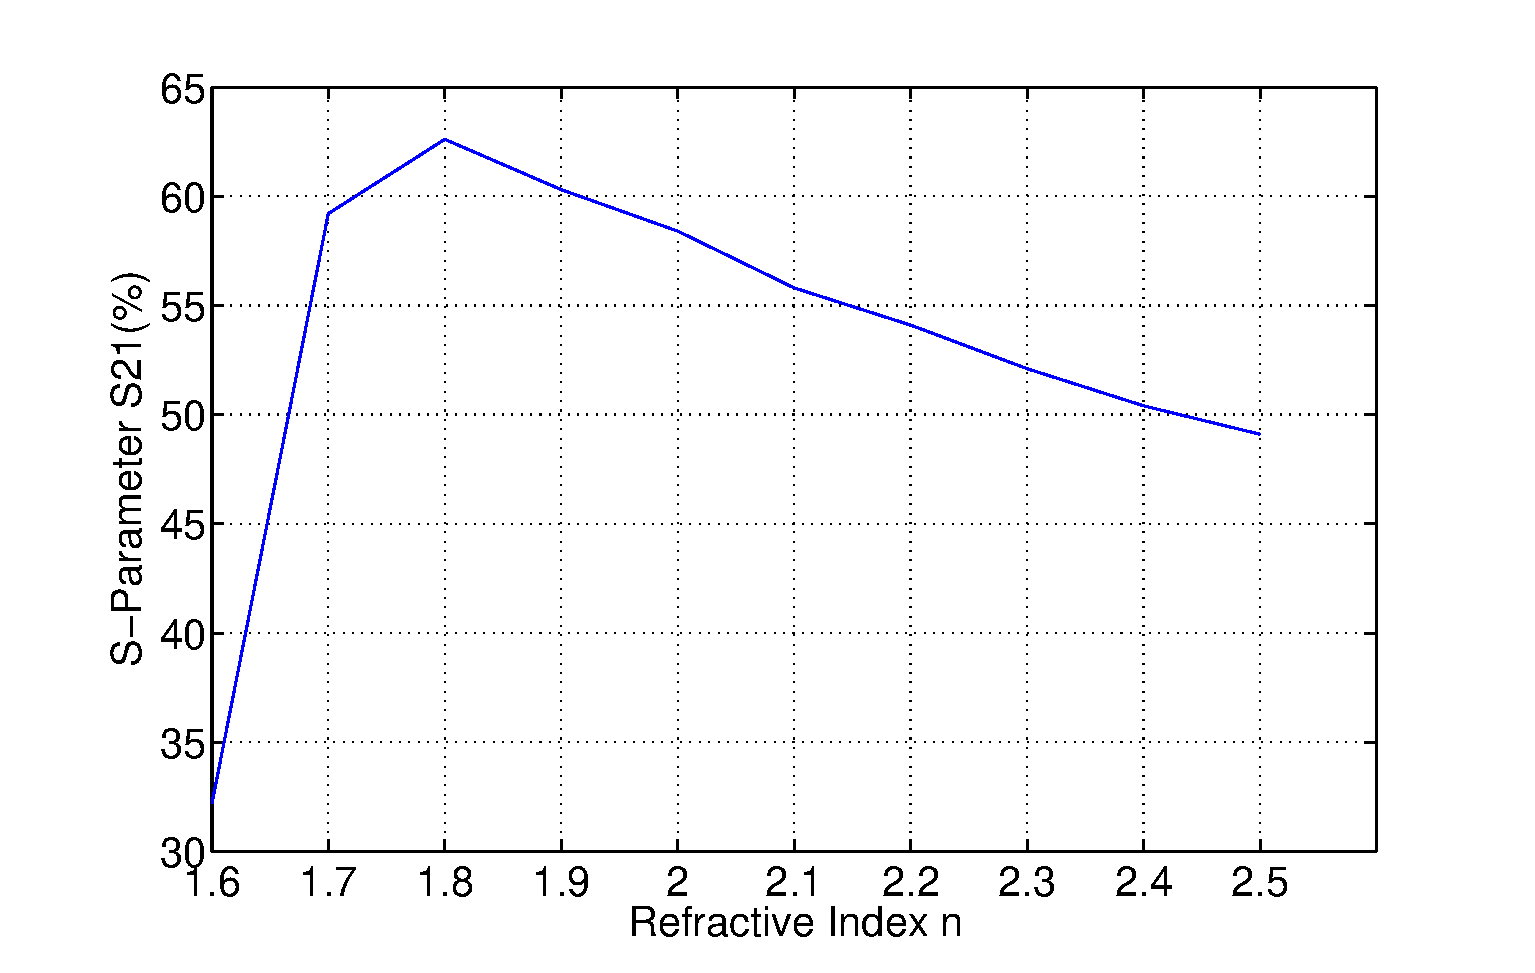
\includegraphics[width=0.7\textwidth]{bilder/s21_refractive_index}
\caption{Coupling efficiency between TLF and the rib waveguide at $f=282$THz due to refractive index.}
\label{fig:refractive_index}
\end{figure}
Simulation results are mapped into Fig. \ref{fig:refractive_index}. It can be told from the figure that the coupling ability rise sharply within $n=1.6$ to $1.8$ then decline softly due to the increasing of refractive indexes. The highest value of the coupling efficiency among the arrangements in this section is about $62.6\%$ when the guide is composed of material of $n=1.8$.\\

Surely, it is not possible to find the material of any refractive index. If we want to improve the coupling ability by this means, we can only choose a material with a refractive index close to $n=1.8$.
